\renewcommand{\arraystretch}{1}
\setlength{\tabcolsep}{7pt}

\chapter{Hyperparameters
selection}\label{appendix---hyperparameters-selection}

In this chapter, we reported the experiments that we run on the
\lmttfont{3DIrcad-dB} to find the best sets of hyperparameters for the tumor
segmentation networks.

Here is the list of hyperparameters to set in our case:

\begin{itemize}
\item
  Learning rate
\item
  Decay
\item
  Number of epochs
\item
  Depth of the network, modelized in our case by the number of filters
  used in the bottleneck of our U-Net architecture
\item
  Initial image size
\item
  Type and amount of data augmentation
\item
  Dropout
\item
  Input type, either single slice or 2.5D
\end{itemize}

Several techniques exist for the determination of the best set of
hyperparameters, such as the grid search or the bayesian hyperparameters
optimization. However given the number of hyperparameters and the time
required to perform one training, it would have been too costly to
implement those techniques that better suits small architectures and
less complex problems, so we have decided to follow an heuristic
approach to find the best set of parameters.\\
We first tried to set the best pairs of learning rate and decay, by
freezing the rest of the parameters. For the chosen optimizer, the
learning rate and the decay will determine how the gradient descent is
performed. A too large initial learning rate will cause the network to
continuously overshoot the minimum, whereas a too small one will require
a large amount of iterations to reach the minimum, as depicted in the figure \ref{fig:gradientDescent}
hereafter.

\begin{figure}
\centering
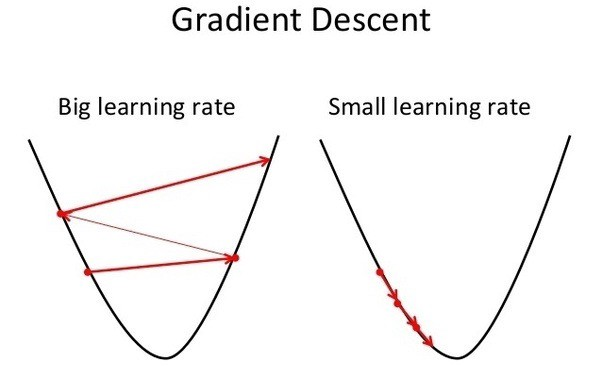
\includegraphics[width=0.5\linewidth]{Appendix/images/media/image1}
\caption{Illustration of the gradient descent when the learning rate is too large (left) or too small (right)}
\label{fig:gradientDescent}
\end{figure}


Once the best candidates were found, we tried to modify the depth of the
network. In the case of the U-Net architecture, one easy way to change
the depth of the network is to add or remove one stage in both the
encoding and the decoding parts. This can be directly modeled by the
number of filters used in the bottleneck part of the network (originally
1024).
In our case, using 1024 filters in the bottleneck part of the network,
will correspond to an architecture with almost 32M parameters.
Setting these first 3 parameters (learning rate, the decay and the depth
of the network) gave us a baseline segmentation accuracy that we tried
to improve with the data augmentation.
As exposed previously, the standard way to apply data augmentation is to
perform geometrical transformations to the original images so that the
network will further be invariant to those modifications.\\
The classical transformations applied are:

\begin{itemize}
\item Translation: Each translation is performed in one randomly chosen
  direction, where the delta value corresponds to the amplitude of the
  shift in terms of number of pixels (e.g shift of 0.1 for an initial
  size of 256 corresponds to a shift of 26 pixels in one direction).
\item Flip : Horizontal or Vertical flip of the original image.
\item Rotation : Apply a rotation of a given angle to the original image.
\end{itemize}

We decided in our case to only investigate the data augmentation that
will prevent the aspect of the liver and its internal tissues. In the
case of elastic deformation, we can not testify that the retained
features will still be discriminant in our deep radiomics approach for
the grade classification if the aspect of the internal liver tissues is
changed.
We have performed for each of the following experiments a 5-Fold
Cross-Validation training on the \lmttfont{3DIrcad-dB}, and the reported results
correspond to the mean slice-wise dice for the given region (
parenchyma or lesion). 


%\section{Parenchyma - Tumor Network Hyperparameters
%}\label{parenchyma---tumor-network-hyperparameters}

\section{Learning Rate \& Decay}\label{learning-rate-decay}

We first evaluated the best pairs of \textbf{learning rate} and
\textbf{decay} when the other parameters such as the number of epochs or
the depth of the network are fixed.

Here are the results obtained with the following fixed parameters:

\begin{itemize}
\item
  Optimizer: Adam
\item
  Number of epochs: 10
\item
  Number of filters at bottleneck: 512
\item
  Input image size: 256
\item
  No data augmentation
\end{itemize}

\begin{table}[!htp]\centering
\caption{Parenchyma segmentation results}
\scriptsize
\begin{tabular}{lrrrrrrr}\toprule
 & &\multicolumn{5}{c}{\textbf{Decay}} \\\cmidrule{3-7}
& &\bm{$ 10^{-1} $} &\bm{$ 10^{-2} $} &\bm{$ 10^{-3} $} &\bm{$ 10^{-4} $} &\bm{$ 10^{-5} $} \\\midrule
\multirow{3}{*}{\textbf{Lr}} &\bm{$ 10^{-3} $} &82.9 &91.9 &90 &80.3 &9.6 \\
&\bm{$ 10^{-4} $} &81.3 &90.8 &90.8 &91.9 &93.7 \\
&\bm{$ 10^{-5} $} &32.4 &76.7 &88 &89.1 &89.7 \\
\bottomrule
\end{tabular}
\end{table}


\begin{table}[!htp]\centering
\caption{Tumor segmentation results}
\scriptsize
\begin{tabular}{lrrrrrrr}\toprule
& &\multicolumn{5}{c}{\textbf{Decay}} \\\cmidrule{3-7}
& &\bm{$ 10^{-1} $} &\bm{$ 10^{-2} $} &\bm{$ 10^{-3} $} &\bm{$ 10^{-4} $} &\bm{$ 10^{-5} $} \\\midrule
\multirow{3}{*}{\textbf{Lr}} &\bm{$ 10^{-3} $} &7.9 &23.5 &24.5 &16.1 &1.5 \\
&\bm{$ 10^{-4} $} &6 &15.6 &15.6 &23.6 &21.7 \\
&\bm{$ 10^{-5} $} &5.4 &5.4 &14 &17 &15.2 \\
\bottomrule
\end{tabular}
\end{table}

Since those two metrics are highly related to the number of voxels of
each class, we decided in order to combine them to incorporate the
number of voxels of each one of the two classes to create a new metric
that will help us select the best networks.

\begin{table}[!htp]\centering
\caption{Segmentation results obtained with the combined metric}
\scriptsize
\begin{tabular}{lrrrrrrr}\toprule
 & &\multicolumn{5}{c}{\textbf{Decay}} \\\cmidrule{3-7}
& &\bm{$ 10^{-1} $} &\bm{$ 10^{-2} $} &\bm{$ 10^{-3} $} &\bm{$ 10^{-4} $} &\bm{$ 10^{-5} $} \\\midrule
\multirow{3}{*}{\textbf{Lr}} &\bm{$ 10^{-3} $} &11.6 &\textbf{26.9} &\textbf{27.7} &19.3 &1.9 \\
&\bm{$ 10^{-4} $} &9.7 &19.3 &19.3 &\textbf{27.0} &\textbf{25.2} \\
&\bm{$ 10^{-5} $} &6.7 &8.9 &17.6 &20.5 &18.9 \\
\bottomrule
\end{tabular}
\end{table}


We can see that using a too small initial learning rate (1e-5) will not
be enough, for the given number of iterations, to approach the minimum
during the gradient descent. On the contrary, when the learning rate is
set at a very high value such as 1e-3, with a small decay (1e-5 or lower
in our case), the network continuously overshoots the minima, ending
with a very large loss.

We selected the pairs providing the best accuracy and investigated the
behavior of the gradient descent when slightly changing the depth of the
network.

\section{Network's depth}\label{networks-depth}

Once the pairs of learning rate and decay selected, we have changed the
depth of the network. This setting is controlled in our pipeline by a
parameter called ``bottleneck filters''.

In the above mentioned experiments, this number was set to 512, and we
tried to change it with the following values: \textbf{\{128, 256, 512,
1024\}}.

Here are the reported results for both the segmentation of the
parenchyma and the tumor when changing the depth of the network:

\begin{table}[!htp]\centering
\caption{Parenchyma segmentation results}
\scriptsize
\begin{tabular}{lrrrrrr}\toprule
& &\multicolumn{4}{c}{\textbf{\# Bottleneck filters}} \\\cmidrule{3-6}
\textbf{Lr} &\textbf{Decay} &\textbf{128} &\textbf{256} &\textbf{512} &\textbf{1024} \\\midrule
$ 10^{-3} $ &$ 10^{-2} $ &76.1 &92.1 &91.9 &7.2 \\
$ 10^{-3} $ &$ 10^{-3} $ &76.5 &88.7 &87 &0 \\
$ 10^{-4} $ &$ 10^{-4} $ &87.1 &92.8 &93.9 &\textbf{94.2} \\
$ 10^{-4} $ &$ 10^{-5} $ &89.7 &92.6 &89.9 &93.6 \\
\bottomrule
\end{tabular}
\end{table}

\begin{table}[!htp]\centering
\caption{Tumor segmentation results}
\scriptsize
\begin{tabular}{lrrrrrr}\toprule
& &\multicolumn{4}{c}{\textbf{\# Bottleneck filters}} \\\cmidrule{3-6}
\textbf{Lr} &\textbf{Decay} &\textbf{128} &\textbf{256} &\textbf{512} &\textbf{1024} \\\midrule
$ 10^{-3} $ &$ 10^{-2} $ &18.5 &17.3 &23.5 &2.8 \\
$ 10^{-3} $ &$ 10^{-3} $ &23.5 &22.1 &24.5 &0 \\
$ 10^{-4} $ &$ 10^{-4} $ &14.6 &22 &25.9 &\textbf{27.6} \\
$ 10^{-4} $ &$ 10^{-5} $ &12.2 &19 &15.2 &26 \\
\bottomrule
\end{tabular}
\end{table}

\begin{table}[!htp]\centering
\caption{Segmentation results obtained with the combined metric}
\scriptsize
\begin{tabular}{lrrrrrr}\toprule
& &\multicolumn{4}{c}{\textbf{\# Bottleneck filters}} \\\cmidrule{3-6}
\textbf{Lr} &\textbf{Decay} &\textbf{128} &\textbf{256} &\textbf{512} &\textbf{1024} \\\midrule
$ 10^{-3} $ &$ 10^{-2} $ &21.3 &21.0 &26.9 &3.0 \\
$ 10^{-3} $ &$ 10^{-3} $ &26.1 &25.4 &27.6 &0.0 \\
$ 10^{-4} $ &$ 10^{-4} $ &18.2 &25.5 &29.2 &\textbf{30.9} \\
$ 10^{-4} $ &$ 10^{-5} $ &16.0 &22.6 &18.9 &29.3 \\
\bottomrule
\end{tabular}
\end{table}

We can see that a too large network depth can cause problems, probably
because the size of the training dataset is too small.

For the next experiments, we have decided to fix the learning rate to
\textbf{1e-4} and the decay to \textbf{1e-4}, with a number of filters
at the bottleneck stage of the network of \textbf{1024}, similar to the
original architecture \cite{Ronneberger2015}.

Once those hyperparameters were set, we investigated the amount and the
type of data augmentation to apply during the training.

\section{Data augmentation}\label{data-augmentation}

We investigate the impact of geometrical data augmentation by first
fixing the amount of data augmentation to 4, meaning that each image in
the training set will be used to create 4 new images. The other
hyperparameters are fixed as follow:

\begin{itemize}
\item
  Lr: 1e-4
\item
  Decay: 1e-4
\item
  Optimizer: Adam
\item
  Number of epochs: 10
\item
  Number of filters at bottleneck: 1024
\item
  Input image size: 256
\end{itemize}

\subsection*{Translation }\label{translation}

We first investigated the value brought by translations during the data
augmentation process, by changing the shift from large to small deltas.

Here are the results for each of the chosen sets:

\begin{longtable}[c]{@{}llll@{}}
\toprule
\textbf{Shift delta} & \textbf{Parenchyma} & \textbf{Tumor} &
\textbf{Combined}\tabularnewline
\midrule
\endhead
No Augm. & 94.2 & 27.6 & 30.9\tabularnewline
{[}-0.1, -0.05, ..., 0.1{]} & 94.8 & 32.6 & 35.7\tabularnewline
{[}-0.1, 0, 0.1{]} & 95 & 32.5 & 35.6\tabularnewline
\textbf{{[}-0.2, 0.1, ..., 0.2{]}} & \textbf{95} & \textbf{34.6} &
\textbf{37.6}\tabularnewline
{[}-0.3, 0.2, ..., 0.3{]} & 94.6 & 32 & 35.1\tabularnewline
\bottomrule
\end{longtable}

We can see that all the experiments provided a better accuracy than the
baseline, with a better accuracy obtained for images augmented with a
shift in the range {[}-0.2, 0.2{]}.

\subsection*{Flip}\label{flip}

We also evaluated the value brought by flipped images during the data
augmentation process. Flip can only be performed horizontally or
vertically, thus a maximum of 2 images can be generated for a given
initial image.

Here are the results obtained when generating only flipped images during
the data augmentation process:

\begin{longtable}[c]{@{}llll@{}}
\toprule
\textbf{Flip} & \textbf{Parenchyma} & \textbf{Tumor} &
\textbf{Combined}\tabularnewline
\midrule
\endhead
No Augm. & 94.2 & 27.6 & 30.9\tabularnewline
\textbf{TRUE} & \textbf{94.7} & \textbf{31.6} &
\textbf{34.7}\tabularnewline
\bottomrule
\end{longtable}

We can see here that flip as data augmentation brings a clear value to
the segmentation performances of the network.

\subsection*{Rotation}\label{rotation}

When applying rotation, we have to carefully choose the angles used
during the rotation since too small angles can cause overfitting and too
large angles can be useless because representing unrealistic data.

Here are the results obtained for the chosen rotation sets:

\begin{longtable}[c]{@{}cccc@{}}
\toprule
\textbf{Rotation angle} & \textbf{Parenchyma} & \textbf{Tumor} &
\textbf{Combined}\tabularnewline
\midrule
\endhead
No Augm. & 94.2 & 27.6 & 30.9\tabularnewline
\hline
\textbf{{[}0, 40{]}} & \textbf{94.9} & \textbf{35.9} & \textbf{38.8}\tabularnewline
{[}0, 80{]} & 87.1 & 36 & 38.5\tabularnewline
{[}0, 90{]} & 87.3 & 36.2 & 38.7\tabularnewline
{[}0, 270{]} & 94.6 & 34.7 & 37.6\tabularnewline
\bottomrule
\end{longtable}

Reported results showed that experiments involving training images
obtained after rotations always improved the baseline accuracy of the
network. It is worth noting that rotations performed with angles in the
range {[}0,40{]} gave results slightly better than when larger angles are used.
Given the results of the above mentioned experiments, we have decided
for the data augmentation to generate new images using \textbf{rotations
with an angle included in the interval {[}0, 40{]}°, both horizontal and
vertical flips, and translation in the range {[}-0.2, 0.2{]}}.

These 3 geometrical transformations will randomly be combined for the
next experiments.

%Here is the list of hyperparameters set for the rest of the experiments:
%
%\begin{itemize}
%\item
%  Lr: 1e-4
%\item
%  Decay: 1e-4
%\item
%  Optimizer: Adam
%\item
%  Number of filters at bottleneck: 1024
%\item
%  Input image size: 256
%\item
%  Data augmentation
%  \begin{itemize}
%  \item
%    Rotations with an angle in the interval {[}0, 40{]}
%  \item
%    Translation with a shift in the interval {[}-0.2, 0.2{]}
%  \item
%    Horizontal and vertical flip
%  \end{itemize}
%\end{itemize}

We first investigated what happened when both augmentation functions are
combined, by incrementally increasing the augmentation factor, and
reported the results hereafter:

\begin{longtable}[c]{@{}ccccc@{}}
\toprule
\textbf{Epochs} & \textbf{Augm. Factor} & \textbf{Parenchyma} &
\textbf{Tumor} & \textbf{Combined}\tabularnewline
\midrule
\endhead
10 & 4 & 94 & 26.6 & 29.9\tabularnewline
10 & 8 & 94.6 & 32.3 & 35.4\tabularnewline
10 & 12 & 94.8 & 34.2 & 37.2\tabularnewline
10 & 16 & 94.9 & 34.9 & 37.9\tabularnewline
10 & 20 & 94.8 & 40.5 & 43.2\tabularnewline
\bottomrule
\end{longtable}

We can see that increasing the number of generated images improves the
segmentation performances of the network.

For this network, we haven't seen any value when adding a dropout with a
rate of 0.2, however this might be discussed because with a higher
number of epochs, the addition of dropout might be beneficial.

\begin{longtable}[c]{@{}cccccc@{}}
\toprule
\textbf{Epochs} & \textbf{Augm. Factor} & \textbf{Dr} &
\textbf{Parenchyma} & \textbf{Tumor} & \textbf{Combined}\tabularnewline
\midrule
\endhead
\textbf{10} & \textbf{20} & \textbf{0} & \textbf{94.8} & \textbf{40.5} & \textbf{43.2}\tabularnewline
10 & 20 & 0.2 & 94.7 & 38.4 & 41.2\tabularnewline
\bottomrule
\end{longtable}

Using the original image size (512x512) seems also to improve the
accuracy of the network, but in these experiments, we trained our
networks with a reduced resolution (256x256) to reduce the training
time.

\begin{longtable}[c]{@{}cccccc@{}}
\toprule
\textbf{Epochs} & \textbf{Augm. Factor} & \textbf{ImgSize} &
\textbf{Parenchyma} & \textbf{Tumor} & \textbf{Combined}\tabularnewline
\midrule
\endhead
10 & 20 & 256 & 94.8 & 40.5 & 43.2\tabularnewline
\textbf{10} & \textbf{20} & \textbf{512} & \textbf{95.1} & \textbf{42.7} & \textbf{45.3}\tabularnewline
\bottomrule
\end{longtable}

We finally increased the number of training epochs, and changed the
augmentation factor, to realize that the best accuracy was obtained with
an augmentation factor of 20 and a network trained with 30 epochs.

Augmenting the data with a factor higher than 20 (e.g 24 in the table
below) tends not to improve the performances of the network. The same
phenomenon is observed when the number of training epochs is increased
at more than 30, probably because the network will start to overfit, due
to a too large number of training iterations, or due to the presence of
images that are too similar.

\begin{longtable}[c]{@{}cccccc@{}}
\toprule
\textbf{Epochs} & \textbf{Augm. Factor} & \textbf{ImgSize} &
\textbf{Parenchyma} & \textbf{Tumor} & \textbf{Combined}\tabularnewline
\midrule
\endhead
10 & 20 & 256 & 94.8 & 40.5 & 43.2\tabularnewline
20 & 16 & 256 & 95 & 43.4 & 45.9\tabularnewline
30 & 16 & 256 & 95.1 & 43.2 & 45.8\tabularnewline
20 & 20 & 256 & 95 & 41.1 & 43.8\tabularnewline
\textbf{30} & \textbf{20} & \textbf{256} & \textbf{95.1} & \textbf{44.9} & \textbf{47.4}\tabularnewline
36 & 20 & 256 & 95 & 42.8 & 45.4\tabularnewline
30 & 24 & 256 & 95.2 & 44.9 & 47.4\tabularnewline
\bottomrule
\end{longtable}

\textbf{The final set of hyperparameters for the segmentation of both
the parenchyma and the tumor} is the following:

\begin{itemize}
\item
  Lr: 1e-4
\item
  Decay: 1e-4
\item
  Number of epochs: 30
\item
  Optimizer: Adam
\item
  Number of filters at bottleneck: 1024
\item
  Input image size: 256
\item
  Data augmentation
  \begin{itemize}
  \item
    Rotations in the interval {[}0, 40{]}
  \item
    Horizontal and vertical flip
  \end{itemize}
\item
  Augmentation factor: 20
\end{itemize}


\renewcommand{\arraystretch}{5}
